\chapter{Cordes, gravité, compactification et T-dualité}

\lectureoverview{Une particule ponctuelle peut se déplacer de façon cohérente sur presque toute géométrie lisse, mais ce n’est pas le cas d’une corde quantique. Ses oscillations de point zéro, en nombre infini, sondent l’espace cible à des échelles toujours plus courtes, et la géométrie effective change à mesure que ces oscillations sont rétablies. Exiger que ce processus atteigne un point fixe conduit à \(R_{\mu\nu}=0\), l’équation d’Einstein dans le vide. Nous passons ensuite de cette condition de cohérence à la compactification. Un cercle fournit à la fois des états de quantité de mouvement de Kaluza--Klein et des états d’enroulement de la corde ; leur échange identifie un cercle de rayon \(R\) à un cercle de rayon \(\alpha'/R\).}

\section{La cohérence comme principe de sélection}

Deux questions se posent. Pourquoi la gravité apparaît-elle dans la théorie des cordes, et pourquoi celle-ci est-elle beaucoup moins permissive que la mécanique des particules ponctuelles ? En réalité, ces deux questions n’en font qu’une. Une géométrie de fond n’est acceptable que si une corde peut s’y propager sans que la théorie conserve une dépendance arbitraire à la finesse avec laquelle nous la résolvons.

Commençons par le problème de référence : une particule ponctuelle contrainte à se déplacer sur une surface courbe lisse. Classiquement, elle suit une géodésique, l’analogue intrinsèque d’une ligne droite. On peut approximer le mouvement par une succession de petits segments, écrire une équation aux différences, puis faire tendre la longueur des segments vers zéro. On obtient ainsi une équation différentielle ordinaire dont la limite continue est bien définie.

La mécanique quantique modifie la somme sur les histoires, mais pas la conclusion. Au lieu de sélectionner une trajectoire classique, on somme les amplitudes associées aux trajectoires sur la surface. On peut de nouveau découper le temps en petits intervalles ; la limite se décrit de façon équivalente par une équation de Schr\"odinger sur l’espace des configurations courbe. Pour une surface lisse, la limite donne un propagateur et un spectre bien définis.

\begin{figure}[H]
  \centering
  \includegraphics[width=0.72\textwidth]{lecture_09_figure_01.png}
  \caption{Une trajectoire lisse sur la surface et une trajectoire en zigzag issue de la somme quantique découpée en tranches temporelles. Toutes deux restent intrinsèques à la surface cible.}
  \lectureframe{00:05:10}
  \label{fig:l09-particle-paths}
\end{figure}

\begin{classroomqa}
\audiencequestion{Dans l’intégrale de chemin, toutes les trajectoires doivent-elles rester sur la surface ? \lecturetimestamp{00:05:39}}
\lecturerresponse{Oui. La surface est l’espace des configurations de la particule, et non une feuille plongée dans un espace plus vaste que la particule pourrait traverser en prenant un raccourci. Chaque point intermédiaire appartient à la surface, et toutes les longueurs et toutes les actions sont calculées à l’aide de sa métrique intrinsèque.}
\end{classroomqa}

La question correspondante pour une corde est plus difficile. Une corde n’est pas caractérisée uniquement par la position de son centre de masse. Elle porte une tour infinie d’oscillateurs ; améliorer la résolution revient donc à admettre davantage de degrés de liberté dynamiques. La théorie n’est cohérente que si les observables tendent vers une limite lorsque cette tour est rétablie.

\section{La particule ponctuelle sur une sphère}

La sphère est la géométrie courbe la plus simple pour effectuer un test. Soit une sphère de rayon \(R\), sur laquelle nous plaçons d’abord une particule de masse \(m\). Pour un mouvement le long d’un grand cercle,
\begin{equation}
  E=\frac{1}{2}mv^2=\frac{p^2}{2m},
  \qquad
  L=pR.
  \label{eq:l09-particle-energy}
\end{equation}
Par conséquent,
\begin{equation}
  E=\frac{L^2}{2mR^2}
   =\frac{L^2}{2I},
  \qquad
  I=mR^2.
  \label{eq:l09-rotor-energy}
\end{equation}
Le rayon intervient par l’intermédiaire du moment d’inertie. La quantification du moment cinétique donne le spectre familier du rotor rigide, sans aucune dépendance à l’égard d’un cutoff ultraviolet.

\begin{figure}[H]
  \centering
  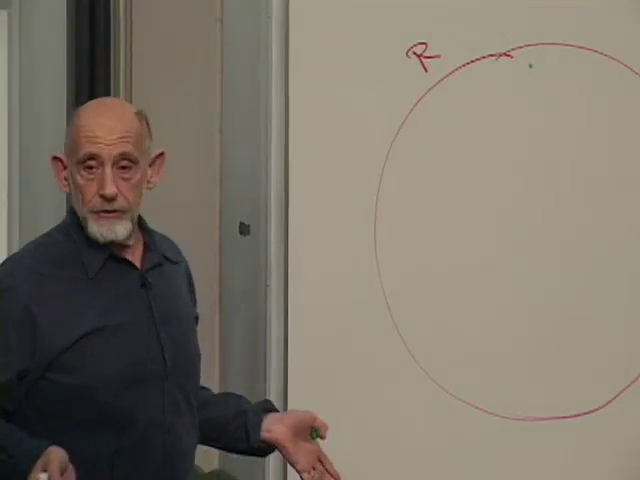
\includegraphics[width=0.74\textwidth]{lecture_09_figure_02.png}
  \caption{Le calcul de référence pour la particule ponctuelle : \(p^2/(2m)=L^2/(2mR^2)=L^2/(2I)\).}
  \lectureframe{00:11:25}
  \label{fig:l09-sphere-rotor}
\end{figure}

Cet exemple sans difficulté est important. La courbure en elle-même n’est pas le problème. Celui-ci apparaît lorsque la courbure est couplée à l’extension quantique interne d’une corde.

\section{La corde du vide n’est pas ponctuelle}

Considérons une coordonnée transverse d’une corde ouverte et soustrayons son centre de masse. Le développement en oscillateurs utilisé ici est schématique :
\begin{equation}
  X(\sigma)-X_{\mathrm{cm}}
  \sim
  \sum_{n=1}^{\infty}
  \frac{a_n+a_n^\dagger}{\sqrt n}\cos(n\sigma).
  \label{eq:l09-mode-expansion}
\end{equation}
Les éléments essentiels sont les modes cosinus, les opérateurs d’oscillateur et le facteur \(1/\sqrt n\). Les normalisations exactes n’interviennent pas dans l’argument sur la taille.
\editorialnote{Le développement précis comporte des facteurs de \(\alpha'\) dépendant des conventions, des constantes numériques et un choix de notation pour les oscillateurs. L’équation \eqref{eq:l09-mode-expansion} ne conserve que la dépendance nécessaire à l’estimation ultraviolette, comme dans le calcul au tableau.}

\begin{figure}[H]
  \centering
  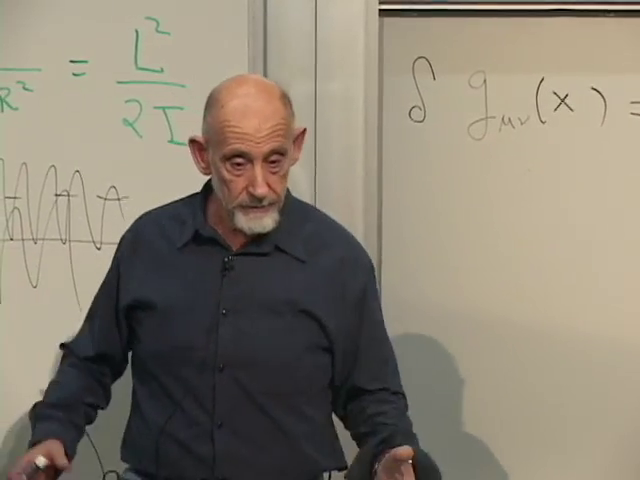
\includegraphics[width=0.78\textwidth]{lecture_09_figure_03.png}
  \caption{Le développement structurel en oscillateurs et la double somme obtenue en l’élevant au carré.}
  \lectureframe{00:15:20}
  \label{fig:l09-string-modes}
\end{figure}

La distance au carré au centre de masse, dans le vide des oscillateurs, vaut
\begin{align}
  \expect{\bigl(X(\sigma)-X_{\mathrm{cm}}\bigr)^2}_0
  &\sim
  \sum_{n,m\geq1}
  \frac{\cos(n\sigma)\cos(m\sigma)}{\sqrt{nm}}\notag\\
  &\qquad\times
  \bra{0}(a_n+a_n^\dagger)\notag\\
  &\hspace{6em}\times(a_m+a_m^\dagger)\ket{0}.
  \label{eq:l09-size-double-sum}
\end{align}
La plupart des termes s’annulent. Deux opérateurs d’annihilation annihilent le ket ; deux opérateurs de création donnent un état orthogonal au bra ; et un opérateur de création suivi d’un opérateur d’annihilation a également une valeur moyenne nulle dans le vide, dans cet ordre. La contraction qui subsiste est
\begin{equation}
  \bra{0}a_n a_m^\dagger\ket{0}=\delta_{nm}.
  \label{eq:l09-vacuum-contraction}
\end{equation}

\begin{figure}[H]
  \centering
  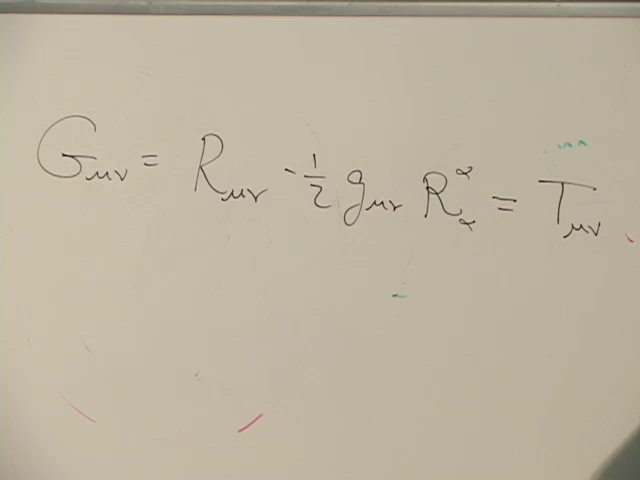
\includegraphics[width=0.74\textwidth]{lecture_09_figure_04.png}
  \caption{La contraction dans le vide qui subsiste réduit la double somme sur les oscillateurs à une somme simple.}
  \lectureframe{00:20:10}
  \label{fig:l09-vacuum-contraction}
\end{figure}

Ainsi,
\begin{equation}
  \expect{\bigl(X(\sigma)-X_{\mathrm{cm}}\bigr)^2}_0
  \sim
  \sum_{n=1}^{\infty}\frac{\cos^2(n\sigma)}{n}.
  \label{eq:l09-size-single-sum}
\end{equation}
En un point générique de la corde, ou après une moyenne sur \(\sigma\), \(\cos^2(n\sigma)\) donne environ \(1/2\). Avec un cutoff sur les modes \(N\),
\begin{equation}
  \expect{\bigl(X-X_{\mathrm{cm}}\bigr)^2}_{0,N}
  \sim
  \frac{1}{2}\sum_{n=1}^{N}\frac{1}{n}
  =\frac{1}{2}\log N+O(1).
  \label{eq:l09-logarithmic-size}
\end{equation}

\begin{figure}[H]
  \centering
  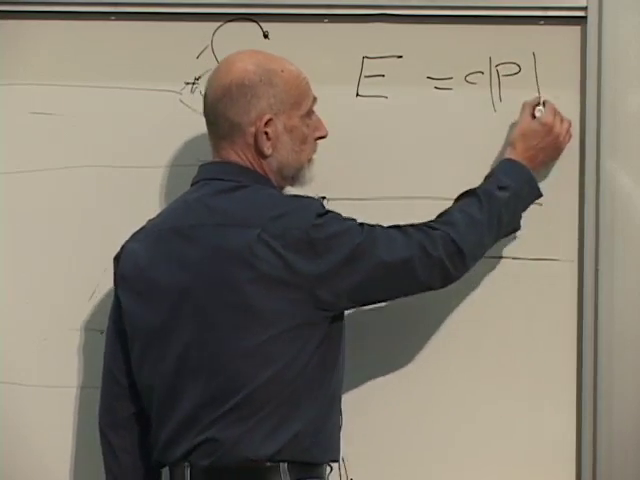
\includegraphics[width=0.72\textwidth]{lecture_09_figure_05.png}
  \caption{Le calcul au tableau aboutit à la somme harmonique qui régit l’étalement de l’état fondamental.}
  \lectureframe{00:22:05}
  \label{fig:l09-harmonic-size}
\end{figure}

En ne conservant, par exemple, que les vingt-cinq premiers modes, on obtient un objet flou de taille finie, mais pas encore la corde continue. La suppression du cutoff fait croître logarithmiquement l’étalement quadratique moyen. Il ne faut pas interpréter cette conclusion comme une preuve de l’incohérence de la théorie des cordes en espace plat. En espace plat, le mouvement du centre de masse et celui des oscillateurs se séparent, et de délicates compensations dans les amplitudes physiques préservent la localité attendue. La croissance de la taille est un signal d’alerte. La courbure nous indique si ce signal annonce une défaillance.

\section{Quand l’étalement interne modifie la géométrie}

Plaçons la corde près du pôle Nord de la sphère. Lorsque tous les oscillateurs sont éteints, elle se comporte comme la particule ponctuelle que nous venons d’étudier. À mesure que l’on admet des modes de plus haute fréquence, la corde devient un enchevêtrement fluctuant qui s’étale sur la calotte. Son centre peut toujours parcourir la sphère, mais l’objet dont le moment d’inertie intervient dans l’énergie de rotation est maintenant étendu.

Pour un axe passant par le centre de la sphère et ses pôles,
\begin{equation}
  I=\int r_\perp^2\,dm,
  \label{eq:l09-extended-inertia}
\end{equation}
où \(r_\perp\) est la distance perpendiculaire d’un élément de corde à cet axe. Un point situé à l’équateur de l’orbite a le bras de levier pertinent le plus grand. Les portions de corde qui retombent vers l’axe contribuent moins. À masse totale fixée, cela diminue le moment d’inertie effectif :
\begin{equation}
  I_{\mathrm{eff}}<mR^2.
  \label{eq:l09-inertia-reduction}
\end{equation}
L’énergie de rotation ressemble donc à celle d’un objet ponctuel sur une sphère plus petite :
\begin{equation}
  E_{\mathrm{rot}}
  =\frac{L^2}{2I_{\mathrm{eff}}}
  \equiv \frac{L^2}{2mR_{\mathrm{eff}}^2},
  \qquad R_{\mathrm{eff}}<R.
  \label{eq:l09-effective-radius}
\end{equation}

\begin{classroomqa}
\audiencequestion{Pourquoi le moment d’inertie devrait-il tendre vers zéro si la corde s’étale sur une région plus vaste ? \lecturetimestamp{00:33:23}}
\lecturerresponse{Il s’agit ici de la description effective après des coarse-grainings successifs, et non de prétendre que la distribution étendue brute a immédiatement un moment d’inertie nul. La première bande de modes transforme le point en une masse floue qui se comporte comme si elle vivait sur une sphère plus petite. La bande suivante résout la structure à l’intérieur de chacune de ces masses et répète le même processus de renormalisation. La répétition de cette comparaison fait décroître le rayon effectif.}
\end{classroomqa}

\begin{figure}[H]
  \centering
  \includegraphics[width=0.72\textwidth]{lecture_09_figure_06.png}
  \medskip

  \begin{adjustbox}{max width=\linewidth}
  \begin{tikzpicture}[x=1cm,y=1cm,>=Latex]
    \draw[thick] (0,0) circle (2.15);
    \draw[dashed] (0,-2.55) -- (0,2.55);
    \draw[blue!65!black,thick]
      (-0.22,2.05)
      .. controls (-1.22,1.75) and (-1.52,1.08) .. (-1.06,0.44)
      .. controls (-0.55,-0.10) and (0.35,0.02) .. (1.10,0.68)
      .. controls (1.48,1.12) and (1.16,1.80) .. (0.20,2.05);
    \draw[red!70!black,dashed] (0,0) circle (1.25);
    \draw[->] (2.70,1.55) -- (4.05,1.55);
    \node[align=center] at (3.37,1.98) {add shorter\\modes};
    \draw[thick] (6.15,0) circle (1.25);
    \draw[dashed] (6.15,-1.65) -- (6.15,1.65);
    \draw[blue!65!black,thick]
      (6.00,1.18)
      .. controls (5.42,0.88) and (5.46,0.25) .. (6.02,-0.06)
      .. controls (6.46,-0.28) and (6.90,0.45) .. (6.28,1.18);
    \node at (0,-3.00) {sphere of radius \(R\)};
    \node at (6.15,-2.05) {effective radius \(R_{\mathrm{eff}}\)};
  \end{tikzpicture}
  \end{adjustbox}
  \caption{La corde près du pôle Nord dessinée au tableau et une reconstruction claire de l’argument du rayon effectif. Le cercle intérieur en pointillés représente une géométrie effective, et non une seconde coquille physique à l’intérieur de la sphère.}
  \lectureframe{00:35:15}
  \label{fig:l09-shrinking-sphere}
\end{figure}

C’est un énoncé de groupe de renormalisation. Un cutoff fini fait de la corde une masse dont la résolution interne est finie. Augmenter le cutoff modifie la mécanique de cette masse. Sur une sphère à courbure positive, chaque couche de modes ajoutée réduit la taille du fond que l’on déduit du mouvement à grande distance. Si le résultat ne se stabilise jamais, il n’existe pas de théorie des cordes indépendante du cutoff sur ce fond.

\section{La métrique doit atteindre un point fixe}

Remplaçons maintenant la sphère par une métrique générale de l’espace cible \(g_{\mu\nu}(x)\). L’intégration d’une fine couche logarithmique de modes d’oscillateur modifie cette métrique par un tenseur local symétrique de rang deux. Cette variation doit s’annuler en espace plat et commencer par des termes à deux dérivées de la métrique. Au premier ordre, la covariance laisse le tenseur de Ricci comme candidat pertinent :
\begin{equation}
  \frac{\partial g_{\mu\nu}}{\partial\log\Lambda}
  =-C\,R_{\mu\nu}+\cdots ,
  \qquad C>0
  \label{eq:l09-ricci-flow}
\end{equation}
dans le sens du coarse-graining utilisé dans l’argument géométrique. Une courbure positive fait alors décroître le rayon d’une sphère, comme requis.
\editorialnote{La normalisation et le signe dépendent du fait que le paramètre de renormalisation augmente vers l’ultraviolet ou vers l’infrarouge. Dans la notation conventionnelle sur la feuille d’univers, la fonction bêta métrique au premier ordre est \(\beta^g_{\mu\nu}=\alpha'R_{\mu\nu}+\cdots\). L’énoncé invariant utilisé ici est que l’indépendance à l’égard du cutoff exige l’annulation de la fonction bêta et donc, à cet ordre, de \(R_{\mu\nu}\).}

\begin{figure}[H]
  \centering
  \includegraphics[width=0.76\textwidth]{lecture_09_figure_07.png}
  \caption{La variation de la métrique est représentée schématiquement par l’opposé du tenseur de Ricci, avec une courbe d’adoucissement dessinée à côté.}
  \lectureframe{00:43:00}
  \label{fig:l09-ricci-flow-board}
\end{figure}

\begin{classroomqa}
\audiencequestion{Où le cutoff des oscillateurs \(N\) intervient-il dans cette équation d’évolution ? \lecturetimestamp{00:43:38}}
\lecturerresponse{C’est la variable d’échelle. La somme qui détermine la taille de la corde varie logarithmiquement lorsque le mode maximal inclus change ; le paramètre d’évolution naturel est donc \(\log N\), ou, de façon équivalente, \(\log\Lambda\). L’équation \eqref{eq:l09-ricci-flow} décrit la variation infinitésimale due à une couche logarithmique de modes.}
\end{classroomqa}

Un fond admissible est un point fixe de cet écoulement. Au premier ordre,
\begin{equation}
  \boxed{R_{\mu\nu}=0.}
  \label{eq:l09-ricci-flat}
\end{equation}
Ricci-plat ne signifie pas que toutes les composantes du tenseur de Riemann s’annulent. Les ondes gravitationnelles, par exemple, peuvent présenter une courbure non nulle dans le vide tout en vérifiant \(R_{\mu\nu}=0\).

\subsection{La même condition est l’équation d’Einstein dans le vide}

En omettant les constantes conventionnelles, l’équation d’Einstein s’écrit
\begin{equation}
  G_{\mu\nu}
  \equiv
  R_{\mu\nu}-\frac12 g_{\mu\nu}R
  =T_{\mu\nu}.
  \label{eq:l09-einstein}
\end{equation}

\begin{figure}[H]
  \centering
  \includegraphics[width=0.78\textwidth]{lecture_09_figure_08.png}
  \caption{Le tenseur d’Einstein et le tenseur énergie-impulsion au tableau.}
  \lectureframe{00:47:15}
  \label{fig:l09-einstein-board}
\end{figure}

Dans le vide, \(T_{\mu\nu}=0\). En prenant la trace en \(D\) dimensions d’espace-temps, on obtient
\begin{equation}
  0=g^{\mu\nu}G_{\mu\nu}
   =\left(1-\frac{D}{2}\right)R.
  \label{eq:l09-einstein-trace}
\end{equation}
Pour \(D\neq2\), on a \(R=0\), et la substitution dans \eqref{eq:l09-einstein} donne \(R_{\mu\nu}=0\). Ainsi, la condition selon laquelle la corde doit perdre sa dépendance au cutoff est l’équation du champ gravitationnel dans le vide. La gravité n’a pas été ajoutée à la théorie : elle apparaît comme le prix de la cohérence.

Le mot \emph{vide} ne signifie pas qu’il ne se passe rien. Il signifie qu’il n’y a pas de source d’énergie-impulsion dans la région. Les équations de Maxwell sans source admettent des ondes électromagnétiques, et les équations d’Einstein sans source admettent des ondes gravitationnelles. La géométrie peut être dynamique même lorsque son tenseur de Ricci s’annule.

\begin{classroomqa}
\audiencequestion{Cette condition est-elle liée à l’invariance conforme ?
\lecturetimestamp{00:52:20}}
\lecturerresponse{Oui, bien que l’enregistrement ne permette que partiellement de saisir la question. La symétrie pertinente est l’invariance conforme de la théorie quantique sur la \emph{feuille d’univers}. Exiger l’annulation de l’anomalie d’échelle sur la feuille d’univers revient à imposer l’annulation de la fonction bêta métrique. Il ne faut pas confondre cela avec l’exigence d’invariance conforme de l’espace-temps lui-même.}
\end{classroomqa}

Il existe une seconde condition de cohérence. L’invariance conforme sur la feuille d’univers fixe aussi la dimension critique de l’espace-temps : dix pour les supercordes et vingt-six pour la corde bosonique. La platitude de Ricci ne constitue donc pas la liste complète des exigences, mais c’est la condition qui fait apparaître le plus directement l’équation d’Einstein.

\section{Des dimensions compactes plutôt que des dimensions manquantes}

Un fond de supercordes comporte neuf dimensions spatiales et une dimension temporelle. Notre monde macroscopique ne présente que trois grandes directions spatiales ; six dimensions spatiales doivent donc être cachées ou rendues autrement inaccessibles aux échelles ordinaires. La compactification les conserve comme de véritables directions, tout en leur donnant une étendue finie et petite.

\begin{classroomqa}
\audiencequestion{Si différents observateurs ont des horloges différentes, cela revient-il à avoir plus d’une dimension temporelle ? \lecturetimestamp{00:56:59}}
\lecturerresponse{Non. Plusieurs horloges sont plusieurs instruments qui mesurent des coordonnées dans un seul espace-temps ; elles ne créent pas des directions temporelles indépendantes. Les dimensions supplémentaires envisagées ici sont spatiales. Les constructions quantiques et causales usuelles ne fournissent pas de théorie cohérente comparable comportant plusieurs directions temporelles locales ; cette possibilité ne fait donc pas partie de ce modèle de compactification.}
\end{classroomqa}

Imaginons des êtres qui pensent que leur monde est une ligne. À faible résolution, ils ne peuvent se déplacer que vers l’avant ou vers l’arrière. Mais sous un microscope suffisamment puissant, la ligne se révèle être un cylindre très fin. Un petit être peut se déplacer autour de sa direction circulaire autant que le long de sa longueur. Cette seconde direction a toujours été présente ; sa circonférence était trop petite pour que les sondes à faible résolution puissent la distinguer.

\begin{figure}[H]
  \centering
  \includegraphics[width=0.78\textwidth]{lecture_09_figure_09.png}
  \caption{Un cylindre étroit et des trajectoires qui s’enroulent autour de sa direction circulaire cachée.}
  \lectureframe{01:01:00}
  \label{fig:l09-hidden-cylinder}
\end{figure}

On peut représenter un cylindre par une bande dont les bords supérieur et inférieur sont identifiés. Le passage par le bord supérieur ramène au bord inférieur à la même position longitudinale. Aucun des deux bords n’est une frontière physique. On peut effectuer la même opération dans deux directions : identifier les bords gauche et droit d’un rectangle, ainsi que ses bords supérieur et inférieur. On obtient alors un tore à deux dimensions.

\begin{figure}[H]
  \centering
  \includegraphics[width=0.76\textwidth]{lecture_09_figure_10.png}
  \medskip

  \begin{tikzpicture}[x=0.82cm,y=0.82cm,>=Latex]
    \draw[thick] (0,0) rectangle (4,2.15);
    \draw[blue!65!black,->] (0,2.48) -- (4,2.48);
    \draw[blue!65!black,->] (4,-0.34) -- (0,-0.34);
    \node at (2,-0.82) {one periodic direction};
    \draw[thick] (6.1,0) rectangle (10.1,2.15);
    \draw[blue!65!black,->] (6.1,2.48) -- (10.1,2.48);
    \draw[blue!65!black,->] (10.1,-0.34) -- (6.1,-0.34);
    \draw[red!70!black,->] (5.76,0) -- (5.76,2.15);
    \draw[red!70!black,->] (10.44,2.15) -- (10.44,0);
    \node at (8.1,-0.82) {two periodic directions};
  \end{tikzpicture}
  \caption{Le parallélépipède dessiné au tableau et une description claire par domaine fondamental. L’identification d’une paire de bords donne un cylindre ; celle des deux paires donne un tore.}
  \lectureframe{01:04:40}
  \label{fig:l09-periodic-identification}
\end{figure}

Le tore est d’abord un objet topologique, avant d’être une surface en forme de beignet dans l’espace à trois dimensions. Si l’on coupe un tore une fois, il devient un cylindre ; si l’on le coupe une seconde fois, il devient un rectangle, à condition de conserver les identifications de bords. On peut munir ce rectangle d’une métrique plate ; le tore plat ainsi obtenu a une courbure de Riemann localement nulle et est donc bien Ricci-plat.

Une trajectoire droite sur le rectangle se poursuit en ligne droite lorsqu’elle traverse un bord identifié. Si sa pente est le rapport rationnel des deux périodes, elle finit par se refermer. Si ce rapport est irrationnel, elle ne se referme jamais et devient dense sur le tore.

\begin{figure}[H]
  \centering
  \includegraphics[width=0.76\textwidth]{lecture_09_figure_11.png}
  \caption{Dans un domaine fondamental, des segments droits répétés représentent une seule trajectoire ininterrompue sur le tore.}
  \lectureframe{01:11:00}
  \label{fig:l09-torus-trajectory}
\end{figure}

On construit les tores de dimension supérieure de la même façon. Un cube dont chaque paire de faces opposées est identifiée forme un tore à trois dimensions, et six directions compactes peuvent être modélisées par un tore à six dimensions. Il ne faut pas chercher à plonger tous ces objets dans l’espace ordinaire à trois dimensions : la description par identification des faces est intrinsèque et complète.

\begin{classroomqa}
\audiencequestion{Une dimension supplémentaire doit-elle nécessairement se refermer sur elle-même ?
\lecturetimestamp{01:15:03}}
\lecturerresponse{Ce n’est pas un théorème. Elle pourrait être non compacte, mais elle apparaîtrait alors normalement comme une autre grande direction dans le monde observé à longue distance. La compacité est le moyen le plus simple de concilier les dimensions supplémentaires avec leur absence apparente. La raison pour laquelle la nature choisirait une compactification particulière relève d’une question dynamique distincte.}
\end{classroomqa}

\begin{classroomqa}
\audiencequestion{Pourquoi supposer que les dimensions invisibles sont des directions spatiales ordinaires enroulées de cette façon, plutôt qu’autre chose ? \lecturetimestamp{01:15:51}}
\lecturerresponse{Parce qu’il s’agit d’une hypothèse précise et soluble, et non parce qu’il aurait été démontré qu’elle est l’unique description de la nature. Les variétés spatiales compactes nous permettent de construire des exemples cohérents et d’en calculer les spectres. Les possibilités plus exotiques doivent justifier leur intérêt en permettant les mêmes calculs.}
\end{classroomqa}

\begin{classroomqa}
\audiencequestion{Les distances sur le tore familier en forme de beignet ne ressemblent pas à celles d’un rectangle. De quelle géométrie s’agit-il ?
\lecturetimestamp{01:18:11}}
\lecturerresponse{Le terme \emph{tore} fixe les identifications, mais pas une métrique unique. Le beignet plongé hérite d’une métrique courbe de l’espace à trois dimensions. Le rectangle dont les bords sont identifiés périodiquement porte une métrique plate. Ils ont la même topologie, mais des géométries différentes ; pour la compactification simple, nous entendons le tore plat.}
\end{classroomqa}

\section{Les paramètres de forme d’un tore plat}

Même un tore plat à deux dimensions n’est pas unique. Son parallélogramme fondamental possède une aire totale, un rapport d’aspect et un cisaillement. Modifier ces paramètres change les distances et, par conséquent, le spectre, sans modifier la topologie.

\begin{figure}[H]
  \centering
  \includegraphics[width=0.74\textwidth]{lecture_09_figure_12.png}
  \medskip

  \begin{tikzpicture}[x=0.9cm,y=0.9cm,>=Latex]
    \draw[thick] (0,0) rectangle (3.4,2.1);
    \draw[<->] (0,-0.35) -- node[below] {\(L_1\)} (3.4,-0.35);
    \draw[<->] (-0.35,0) -- node[left] {\(L_2\)} (-0.35,2.1);
    \draw[thick] (5.4,0) -- (8.8,0) -- (9.7,2.1) -- (6.3,2.1) -- cycle;
    \draw[dashed] (5.4,0) -- (6.3,2.1);
    \draw[->] (5.75,2.48) -- node[above] {shear} (6.45,2.48);
    \node at (1.7,-1.00) {area and aspect ratio};
    \node at (7.55,-1.00) {complex structure};
  \end{tikzpicture}
  \caption{Les domaines fondamentaux rectangulaire et cisaillé utilisés pour discuter des modules du tore.}
  \lectureframe{01:23:00}
  \label{fig:l09-torus-moduli}
\end{figure}

Pour un tore à deux dimensions, il est commode de regrouper la forme dans un nombre complexe \(\tau=\tau_1+i\tau_2\) : sa partie réelle représente le cisaillement et sa partie imaginaire représente un rapport d’aspect, une fois l’échelle globale séparée. L’échange des deux cycles de base ou un changement de leur base entière peut faire correspondre des parallélogrammes apparemment différents au même tore.

\begin{classroomqa}
\audiencequestion{Que se passe-t-il si l’on retourne un bord avant de l’identifier ? \lecturetimestamp{01:24:20}}
\lecturerresponse{On obtient une topologie différente. Une identification avec réflexion donne une surface non orientable, la bouteille de Klein, plutôt qu’un tore ordinaire.}
\end{classroomqa}

\begin{classroomqa}
\audiencequestion{Et si la torsion n’est pas uniforme le long du bord ?
\lecturetimestamp{01:25:01}}
\lecturerresponse{Une déformation lisse non uniforme peut être transférée à la métrique du domaine fondamental. Il faut distinguer l’identification topologique des données géométriques : modifier le recollement peut changer la topologie, tandis qu’une variation lisse des distances modifie la métrique.}
\end{classroomqa}

\editorialnote{Pour un tore plat à deux dimensions, l’aire est le module de Kähler le plus simple, et \(\tau\) est le module de structure complexe. Un cisaillement continu fait partie de \(\tau\). En revanche, une torsion de Dehn est une opération discrète du groupe des classes de difféomorphismes, représentée par \(\tau\mapsto\tau+1\) ; elle n’est pas en elle-même un module continu. Cette distinction précise une terminologie volontairement informelle employée lors de la discussion au tableau.}

Les tores plats sont utiles, car ils satisfont immédiatement la condition de cohérence, mais leur symétrie est trop généreuse pour un modèle réaliste de la physique des particules. Des espaces Ricci-plats plus complexes, notamment les variétés de Calabi--Yau, offrent des compactifications plus riches. Leur construction détaillée dépasse le cadre de cette discussion ; le principe reste le même.

\section{Lire un cercle compact à partir de son spectre}

Après la pause, réduisons l’espace compact à un cercle de circonférence \(2\pi R\). La fonction d’onde doit être monovaluée après un tour :
\begin{equation}
  e^{ip_c(x+2\pi R)/\hbar}=e^{ip_cx/\hbar}.
\end{equation}
On en déduit
\begin{equation}
  p_cR=n\hbar,
  \qquad
  p_c=\frac{n\hbar}{R},
  \qquad n\in\mathbb Z.
  \label{eq:l09-kk-momentum}
\end{equation}

\begin{figure}[H]
  \centering
  \includegraphics[width=0.74\textwidth]{lecture_09_figure_13.png}
  \caption{La circonférence compacte \(2\pi R\) et la quantité de mouvement quantifiée \(p_c=n\hbar/R\).}
  \lectureframe{01:32:15}
  \label{fig:l09-kk-board}
\end{figure}

Pour une particule sans masse dans l’espace-temps complet,
\begin{equation}
  E=c|\mathbf P|.
  \label{eq:l09-massless-dispersion}
\end{equation}

\begin{figure}[H]
  \centering
  \includegraphics[width=0.70\textwidth]{lecture_09_figure_14.png}
  \caption{La relation de dispersion d’une particule sans masse utilisée pour réinterpréter la quantité de mouvement compacte comme une masse en dimension inférieure.}
  \lectureframe{01:33:45}
  \label{fig:l09-massless-board}
\end{figure}

Séparons les composantes non compactes et compacte de la quantité de mouvement, et posons \(c=\hbar=1\) :
\begin{equation}
  E^2=\mathbf p_{\mathrm{large}}^2+\frac{n^2}{R^2}.
  \label{eq:l09-kk-dispersion}
\end{equation}
Un observateur incapable de résoudre la direction compacte compare cela à \(E^2=\mathbf p_{\mathrm{large}}^2+m^2\) et en déduit une tour de masses
\begin{equation}
  m_n=\frac{|n|}{R}.
  \label{eq:l09-kk-masses}
\end{equation}
Les deux signes de \(n\) correspondent à des quantités de mouvement compactes opposées, associées à la même énergie positive, et non à des masses positives et négatives. L’espacement \(1/R\) révèle donc le rayon par spectroscopie. C’est le mécanisme de Kaluza--Klein : la quantité de mouvement dans une direction cachée apparaît comme une masse dans les dimensions visibles.

\section{Les états d’enroulement complètent le spectre}

Une corde fermée possède une possibilité qui n’existe pas pour une particule ponctuelle : elle peut s’enrouler autour du cercle. Si le nombre d’enroulement est \(w\), la corde ne se referme qu’après avoir parcouru \(w\) fois la direction compacte. Sa longueur est \(2\pi |w|R\) ; la tension lui confère donc une énergie
\begin{equation}
  m_w
  =2\pi T\,|w|R
  =\frac{|w|R}{\alpha'}.
  \label{eq:l09-winding-mass}
\end{equation}
Le cours choisit des unités telles que \(\alpha'=1\), ce qui ramène l’expression à
\begin{equation}
  m_w=|w|R.
  \label{eq:l09-winding-lecture-units}
\end{equation}
Les valeurs positive et négative de \(w\) correspondent à des orientations opposées autour du cercle.

\begin{figure}[H]
  \centering
  \includegraphics[width=0.76\textwidth]{lecture_09_figure_15.png}
  \caption{Une corde fermée enroulée autour du cylindre compact, avec le rayon compact indiqué au tableau.}
  \lectureframe{01:39:45}
  \label{fig:l09-winding-board}
\end{figure}

Le cercle compact produit donc deux tours complémentaires :
\begin{equation}
  m_n=\frac{|n|}{R},
  \qquad
  m_w=\frac{|w|R}{\alpha'}.
  \label{eq:l09-two-towers}
\end{equation}
Lorsque \(R\) est grand, les niveaux de quantité de mouvement sont rapprochés et les états d’enroulement sont lourds. Lorsque \(R\) est petit, les niveaux de quantité de mouvement sont espacés et les états d’enroulement sont légers.

\begin{figure}[H]
  \centering
  \begin{tikzpicture}[x=1cm,y=0.9cm,>=Latex]
    \draw[->] (0,0) -- (0,4.7) node[above] {\(m\)};
    \foreach \y/\lab in {0/0,1.1/{1/R},2.2/{2/R},3.3/{3/R},4.4/{4/R}} {
      \draw (-0.16,\y) -- (0.16,\y);
      \node[left] at (-0.22,\y) {\(\lab\)};
    }
    \node at (0,-0.62) {momentum};
    \draw[<->,very thick,blue!65!black] (2.05,2.15) -- (4.05,2.15)
      node[midway,above] {\(R\leftrightarrow\alpha'/R\)};
    \draw[->] (6.1,0) -- (6.1,4.7) node[above] {\(m\)};
    \foreach \y/\lab in {0/0,1.1/{R/\alpha'},2.2/{2R/\alpha'},3.3/{3R/\alpha'},4.4/{4R/\alpha'}} {
      \draw (5.94,\y) -- (6.26,\y);
      \node[right] at (6.32,\y) {\(\lab\)};
    }
    \node at (6.1,-0.62) {winding};
  \end{tikzpicture}
  \caption{Les tours de quantité de mouvement et d’enroulement s’échangent lorsque le rayon est inversé en unités de corde.}
  \label{fig:l09-dual-mass-towers}
\end{figure}

\section{T-dualité : les petits et les grands cercles décrivent la même physique}

Les deux tours s’échangent selon
\begin{equation}
  R\longleftrightarrow\frac{\alpha'}{R},
  \qquad
  n\longleftrightarrow w.
  \label{eq:l09-t-duality}
\end{equation}
Dans les unités utilisées au tableau, \(\alpha'=1\) ; il s’agit donc simplement de \(R\leftrightarrow1/R\). Au rayon autodual \(R=\sqrt{\alpha'}\), les échelles de quantité de mouvement et d’enroulement coïncident.

\begin{figure}[H]
  \centering
  \includegraphics[width=0.74\textwidth]{lecture_09_figure_16.png}
  \caption{Au tableau, comparaison des spectres de masse clairsemés et denses lorsque le rayon franchit l’échelle autoduale.}
  \lectureframe{01:43:00}
  \label{fig:l09-duality-board}
\end{figure}

L’échange des formules élémentaires de masse n’est que l’aspect visible du résultat. Les états oscillatoires de la corde fermée et les amplitudes de diffusion sont également mis en correspondance de façon cohérente. Un cercle plus petit que l’échelle de la corde ne constitue pas une nouvelle géométrie toujours plus minuscule : il admet une description équivalente par un cercle dual plus grand. Les particules ponctuelles ne permettent pas cette identification, car elles possèdent des modes de quantité de mouvement, mais pas de modes d’enroulement.

\begin{classroomqa}
\audiencequestion{S’agit-il simplement de l’échange d’une direction verticale avec une direction horizontale ? \lecturetimestamp{01:44:38}}
\lecturerresponse{Non. Il s’agit de l’échange de deux nombres quantiques différents : la quantité de mouvement autour du cercle et le nombre de fois qu’une corde fermée s’enroule autour de celui-ci. Le rayon doit être inversé en même temps.}
\end{classroomqa}

\begin{classroomqa}
\audiencequestion{Les descriptions en \(R<\sqrt{\alpha'}\) et \(R>\sqrt{\alpha'}\) concernent-elles uniquement les bosons, ou aussi les fermions ?
\lecturetimestamp{01:46:30}}
\lecturerresponse{La dualité est une symétrie de la théorie des cordes compactifiée complète, et pas seulement du simple spectre de masses bosonique utilisé pour la mettre en évidence. La correspondance détaillée entre les secteurs dépend de la théorie, mais l’équivalence petit--grand ne se limite pas à une seule espèce de particules.}
\end{classroomqa}

\begin{classroomqa}
\audiencequestion{Compare-t-on des cordes ouvertes ou des cordes fermées ? \lecturetimestamp{01:47:32}}
\lecturerresponse{Il s’agit d’états de cordes fermées. Une corde fermée libre peut s’enrouler autour d’un cercle compact. Une corde ouverte ordinaire à extrémités libres ne porte pas le même nombre d’enroulement conservé.}
\end{classroomqa}
\editorialnote{Dans la description plus complète des cordes ouvertes, la T-dualité échange les conditions aux limites de Neumann et de Dirichlet et introduit les D-branes. C’est pourquoi la T-dualité des cordes ouvertes est plus riche qu’une simple reprise de la formule d’enroulement des cordes fermées.}

\begin{classroomqa}
\audiencequestion{Cet échange est-il analogue à celui de l’espace et du temps près de l’horizon d’un trou noir ? \lecturetimestamp{01:48:00}}
\lecturerresponse{Non. Les coordonnées de l’horizon et le caractère causal relèvent d’une autre question. Ici, les deux descriptions portent sur un cercle spatial compact et sur l’échange de ses secteurs de quantité de mouvement et d’enroulement.}
\end{classroomqa}

\begin{classroomqa}
\audiencequestion{Cela résout-il le problème de l’auto-énergie à courte distance en introduisant une longueur minimale ? \lecturetimestamp{01:48:35}}
\lecturerresponse{Cela montre que les rayons inférieurs à l’échelle de la corde ne définissent pas de nouveaux fonds circulaires non équivalents : diminuer \(R\) au-delà du point autodual augmente le rayon dual. Il s’agit d’un obstacle précis, propre aux cordes, à l’exploration d’une géométrie circulaire arbitrairement petite, mais il ne faut pas en conclure que toute notion imaginable de distance possède une limite inférieure universelle et absolue.}
\end{classroomqa}

\section{Pourquoi on ne peut pas omettre les secteurs d’enroulement}

\begin{classroomqa}
\audiencequestion{Pourrait-on définir la théorie en ne considérant que les cordes non enroulées et en excluant les états d’enroulement ? \lecturetimestamp{01:48:56}}
\lecturerresponse{Non. Les interactions entre cordes fermées les engendrent. Étirez une boucle non enroulée autour de la direction compactifiée, de sorte qu’un segment parcoure le cercle dans un sens et un autre dans le sens opposé. L’enroulement net reste nul. Une reconnexion peut alors scinder la boucle en deux cordes fermées d’enroulements \(+1\) et \(-1\). La paire peut se séparer ; les états d’enroulement doivent donc faire partie du spectre, même si l’état initial n’en comportait aucun.}
\end{classroomqa}

\begin{figure}[H]
  \centering
  \includegraphics[width=0.74\textwidth]{lecture_09_figure_17.png}
  \caption{La boucle étirée, d’enroulement nul, disposée autour de la direction compactifiée avant la reconnexion.}
  \lectureframe{01:50:30}
  \label{fig:l09-winding-pair-before}
\end{figure}

\begin{figure}[H]
  \centering
  \includegraphics[width=0.72\textwidth]{lecture_09_figure_18.png}
  \medskip

  \begin{tikzpicture}[x=0.9cm,y=0.9cm,>=Latex]
    \draw[thick] (0,0) ellipse (1.0 and 1.55);
    \draw[blue!65!black,thick]
      (0.08,1.35) .. controls (2.0,1.15) and (2.0,-1.15) .. (0.08,-1.35);
    \draw[red!70!black,thick]
      (-0.08,-1.35) .. controls (-2.0,-1.15) and (-2.0,1.15) .. (-0.08,1.35);
    \node at (0,-2.15) {net \(w=0\)};
    \draw[->,thick] (2.45,0) -- (3.75,0) node[midway,above] {split};
    \draw[thick] (5.05,0.62) ellipse (0.68 and 1.02);
    \draw[blue!65!black,very thick,->]
      (5.05,1.64) arc[start angle=90,end angle=-250,x radius=0.68,y radius=1.02];
    \node at (5.05,-0.82) {\(w=+1\)};
    \draw[thick] (7.45,0.62) ellipse (0.68 and 1.02);
    \draw[red!70!black,very thick,<-]
      (7.45,1.64) arc[start angle=90,end angle=-250,x radius=0.68,y radius=1.02];
    \node at (7.45,-0.82) {\(w=-1\)};
  \end{tikzpicture}
  \caption{La boucle enroulée séparée représentée au tableau et une reconstruction fidèle de la production d’une paire d’enroulement--anti-enroulement. L’enroulement total reste nul.}
  \lectureframe{01:51:30}
  \label{fig:l09-winding-pair-after}
\end{figure}

\begin{classroomqa}
\audiencequestion{La production de la paire d’enroulements nécessite-t-elle de l’énergie supplémentaire ?
\lecturetimestamp{01:52:11}}
\lecturerresponse{Oui. Étendre une corde coûte de l’énergie de tension, et les cordes enroulées finales ont les masses données par
\eqref{eq:l09-winding-mass}. Une collision suffisamment énergétique peut produire la paire, tout comme une collision peut produire une particule et son antiparticule tout en préservant la charge conservée pertinente.}
\end{classroomqa}

\section{Peut-on entendre la forme d’un fond de cordes ?}

Dans une théorie ordinaire des particules compactifiée, l’espacement du spectre de Kaluza--Klein permet d’inférer le rayon : on cherche à entendre la forme de l’espace compact à partir de ses modes normaux. En théorie des cordes, le problème inverse est plus subtil. Les modes de quantité de mouvement révèlent \(1/R\), les modes d’enroulement révèlent
\(R/\alpha'\), et le spectre complet reste inchangé lorsqu’on échange les deux. Deux rayons que la géométrie des particules ponctuelles considère comme distincts correspondent à un seul et même fond de cordes décrit au moyen de variables duales.

Le cours est ainsi parvenu, par une seule voie, aux deux conclusions annoncées. La cohérence ultraviolette impose à la métrique cible de satisfaire l’équation d’Einstein dans le vide ; la gravité est donc inévitable. La compactification transforme ensuite une géométrie cachée en spectres de particules, mais les états d’enroulement empêchent ce spectre d’attribuer un rayon classique unique en dessous de l’échelle des cordes. La cohérence ne détermine pas seulement quelles géométries sont autorisées : par la T-dualité, elle change aussi ce qui compte comme une géométrie distincte.